% ================= 4. METHODOLOGY =================
\section{Methodology}
\label{sec:methodology}

Section~\ref{sec:wbs} assigns every task an owner and a date. This section
states the reasoning that assignment is built on: the procedure the team
follows to take the Cubli from a sizing target to a validated prototype, why
its six stages run in this order and not another, and why the result is an
iteration rather than a single pass through them.

\subsection{Development and Iteration Workflow}
\label{sec:dev_workflow}

Figure~\ref{fig:methodology_workflow} is that procedure: six stages, each
committing an output the next stage cannot start without, and three feedback
paths that reopen an earlier stage when a downstream finding invalidates an
upstream assumption.

\begin{figure}[htbp]
\centering
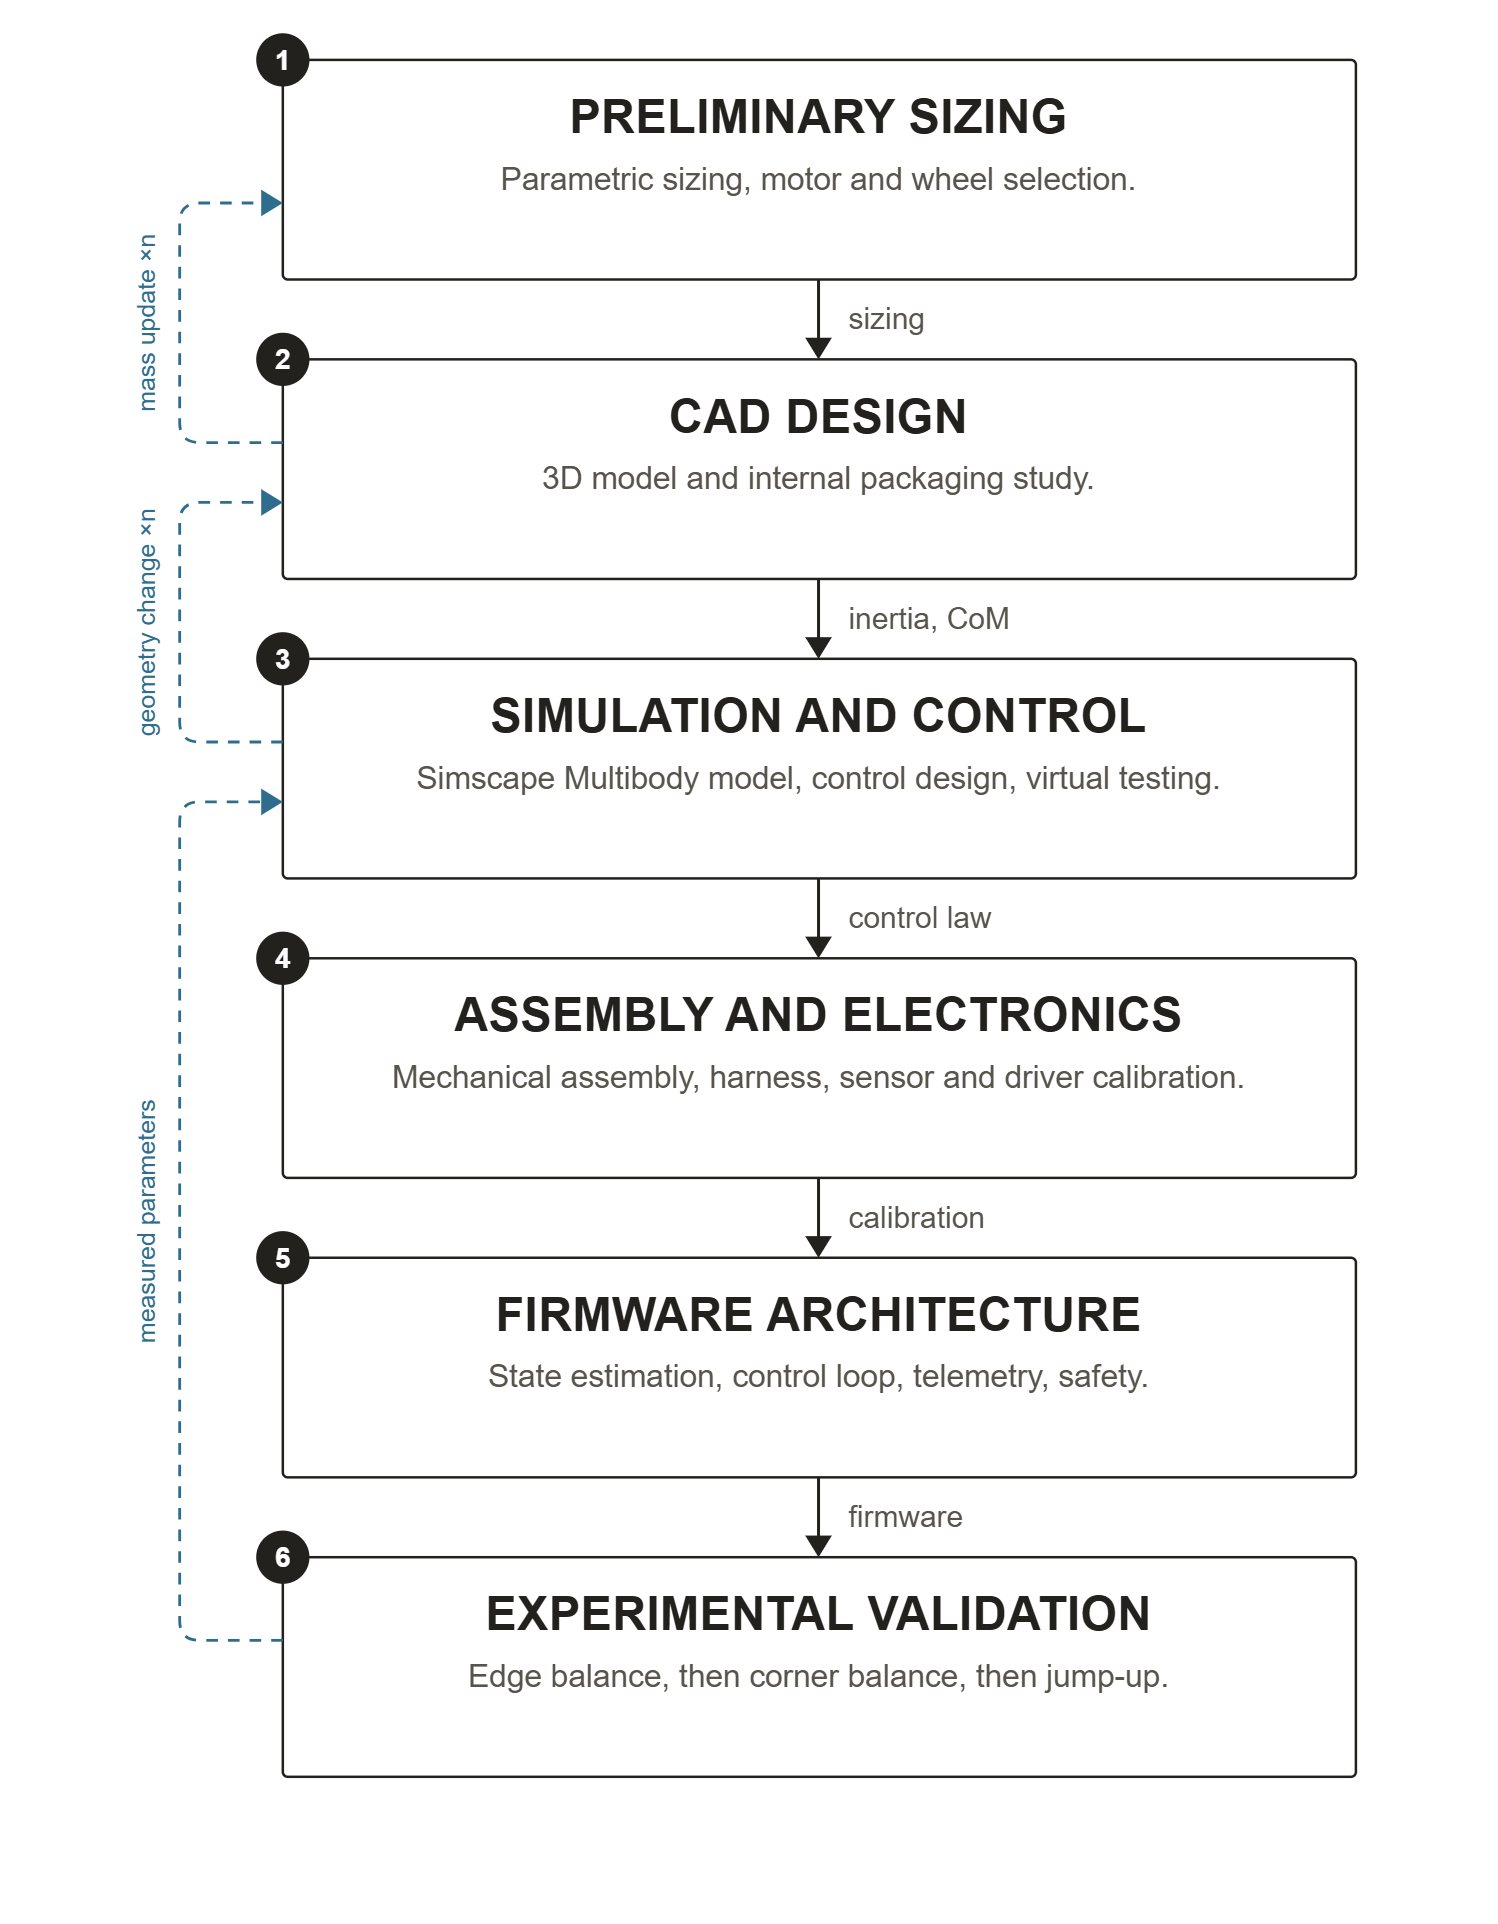
\includegraphics[width=0.8\linewidth]{images/methodology_diagram.png}
\caption[Development and iteration workflow]{Development and iteration
workflow, with the three feedback loops that keep sizing, CAD and control
consistent with each other and with measured hardware.}
\label{fig:methodology_workflow}
\end{figure}

\paragraph{Why this order.} Each stage sits where it does because the stage
after it consumes an output only it produces:
\begin{enumerate}
\item \textbf{Preliminary Sizing} (Section~\ref{sec:sizing}) fixes cube mass,
  edge length and target wheel inertia before anything is drawn, because a
  part modelled to the wrong mass has to be redrawn no matter how well it is
  drawn.
\item \textbf{CAD Design} (Section~\ref{sec:cad}) turns those targets into a
  3D model and an internal packaging study that returns a measured inertia
  tensor and centre of mass --- figures Stage~1 could only estimate.
\item \textbf{Simulation and Control} (Sections~\ref{sec:2dmodel}--\ref{sec:3dmodel},
  \ref{sec:control_algorithms}) is designed against that CAD-derived inertia
  rather than the Stage~1 estimate, since a controller tuned on the wrong
  inertia tensor is validated against the wrong plant.
\item \textbf{Assembly and Electronics} (Section~\ref{sec:electrical}) begins
  only once a control law exists to bring the hardware up against, so the
  first closed-loop command a newly wired axis receives is a designed one
  (Section~\ref{sec:gradual_control}), not an improvised one.
\item \textbf{Firmware Architecture} integrates the calibrated sensors and
  drivers of the previous stage into the estimator and control loop Stage~3
  designed.
\item \textbf{Experimental Validation} (Section~\ref{sec:verification}) is
  last because it is the only stage that checks the previous five against
  reality rather than against each other.
\end{enumerate}

\paragraph{Why it loops.} A single pass through that order is not sufficient,
because three of its outputs correct an assumption made earlier in the same
pass rather than only feeding forward:
\begin{itemize}
\item \emph{Mass update.} CAD's as-modelled mass and CoM close the loop into
  Stage~1's assumed $M$ (Section~\ref{sec:massbudget}), exactly as
  Algorithm~\ref{alg:sizing_closure} states it: the sizing reported there is
  the fixed point of this loop, not its first iteration.
\item \emph{Geometry change.} A control or simulation finding --- inertia
  short of target, an infeasible slew, an interference the 2D model could not
  see --- returns to CAD rather than being absorbed by re-tuning gains, since
  no gain fixes a wheel that does not fit or a body the controller cannot
  actuate against.
\item \emph{Measured parameters.} Once hardware exists, the torque constant,
  friction and latency measured on it (Section~\ref{sec:paramid}) replace the
  CAD/datasheet estimates Stage~3 was designed on, and the control gains are
  re-derived against the measured plant rather than flown on assumed values.
\end{itemize}
This is also why the schedule of Section~\ref{sec:schedule} gates CAD on the
sizing numbers rather than running the two in parallel: a frame frozen ahead
of the inertia tensor is a frame that may have to be reprinted, which costs
more than the days spent waiting on the number.

The full Cubli is underactuated and simultaneously unstable about all three
axes when balanced on a corner (Section~\ref{sec:objectives}). Stage~3 of the
procedure above is therefore itself incremental: a first, single-face 1-DoF
prototype is built and modelled in two dimensions, so that the dynamics, the
parameter identification procedure and the estimator can be validated on a
plant simple enough to reason about directly; the same modelling,
identification and verification workflow is then generalised to the second
and final prototype, the fully three-dimensional cube, in
Section~\ref{sec:3dmodel}. Each subsection below states the equations that
define the problem at that stage and the method used to determine every
parameter that appears in them; the control law itself --- how those
equations are turned into a feedback command --- is derived separately in
Section~\ref{sec:control_algorithms}, since sizing, dynamics and control are
three passes over the same plant rather than three independent problems.

\subsection{Sizing Closure Algorithm}
\label{sec:sizing_algorithm}

The wheel sizing of Section~\ref{sec:massbudget} is not evaluated once: cube
mass, target inertia and wheel design are mutually dependent, and the design
point reported there is the fixed point of an iteration, not the result of a
single pass. Table~\ref{tab:sizing_procedure} states that iteration's six
stages in prose; Algorithm~\ref{alg:sizing_closure} is their formal statement,
as implemented in \texttt{analysis/SIZING.py} and run to convergence by hand.

\begin{algorithm}[htbp]
\caption{Mass--inertia closure procedure (\texttt{analysis/SIZING.py})}
\label{alg:sizing_closure}
\begin{algorithmic}[1]
\Require Initial mass guess $M_0$; fixed inputs $L,\eta,\tau_b,\omega_{\max}$;
  envelope diameter $D_w$; bill-of-materials line items; structure allowance
  $A$; closure tolerance $\varepsilon$
\Ensure Converged cube mass $M^\star$ and wheel design $(D_w,N,m_w,I_w)$
\State $M \gets M_0$
\Repeat
  \State \textit{Stage 1 (jump-up target):} $\tau_g \gets MgL/2$;
    \textbf{abort} if $\tau_b \le \tau_g$ (brake floor violated)
  \State \phantom{\textit{Stage 1:}} $\beta \gets \tau_b/(\tau_b-\tau_g)$;\ \
    $h_w \gets \beta\sqrt{\eta}\,C_{\text{corner}}\,ML^{3/2}$;\ \
    $I_{w,\text{target}} \gets h_w/\omega_{\max}$
  \State \textit{Stage 2 (solid wheel):} evaluate bare ring$+$spoke mass
    $m_{\text{solid}}$ and inertia $I_{\text{solid}}$ at $D_w$
  \State \textit{Stage 3 (per-station increment):} compute net mass $m_b$ and
    net inertia $\Delta I_b$ added by one ballast station at its forced
    centroid radius
  \State \textit{Stage 4 (solve station count):}
    $N \gets \big\lceil (I_{w,\text{target}}-I_{\text{solid}})/\Delta I_b
    \big\rceil$, rounded to the nearest admissible multiple
  \State \textit{Stage 5 (feasibility):} cap $N$ at $N_{\max}$ (edge-gap
    rule); check axial wall clearance and bolt retention load; if no $D_w$ in
    the swept range is feasible, widen the sweep or relax $\omega_{\max}$
  \State \textit{Stage 6 (mass roll-up):} $m_w \gets m_{\text{solid}} +
    N\,m_b$;\ \ $M_{\text{est}} \gets \sum(\text{known BOM}) + 3m_w + A$
  \State $\delta \gets M_{\text{est}} - M$;\qquad $M \gets M_{\text{est}}$
\Until{$|\delta| < \varepsilon$}
\State \Return $M^\star \gets M$,\ $(D_w,N,m_w,I_w)$
\end{algorithmic}
\end{algorithm}

\paragraph{Convergence behaviour.} Because the achievable inertia grows with
$D_w^2$ while the requirement grows with $L^{3/2}$ (Section~\ref{sec:massbudget}),
successive mass estimates approach the fixed point monotonically rather than
oscillating, and because the station count $N$ moves in discrete steps rather
than continuously with $M$, the iteration typically lands on the fixed point
in one or two passes once $N$ stops changing. Table~\ref{tab:convergence_trace}
records the trace for the current design point: starting from the working
guess $M_0=\qty{1.4652}{\kilo\gram}$, the station count is already stable at
the first pass, and the second pass reproduces its own input to
\qty{0.0}{\gram}. The same fixed point is reached from other starting guesses
(cold-started at \qty{1.700}{\kilo\gram}, or from the previous design's
$M=\qty{1.772}{\kilo\gram}$), which is the evidence that the reported point is
a genuine attractor of the iteration rather than an artefact of the starting
guess.

\begin{table}[htbp]
\centering
\caption[Sizing closure convergence trace]{Sizing closure convergence trace
for the converged design point (\qty{374}{\gram} structure allowance).}
\label{tab:convergence_trace}
\small
\begin{tabular}{c c c c c c}
\toprule
Pass & $M$ assumed (kg) & $N$ & $m_w$ (g) & $M_{\text{est}}$ (kg) & $\delta$ (g) \\
\midrule
1 & 1.4652 & 3 & 149.11 & 1.4654 & $+0.2$ \\
2 & 1.4654 & 3 & 149.11 & 1.4654 & $+0.0$ \\
\bottomrule
\end{tabular}
\end{table}

\paragraph{A caution specific to this implementation.} Stage~6 is implemented
as a literal bill of materials, decoupled from Stages~2--5 so that the mass
budget can be edited independently of the wheel model. The consequence is that
the reaction-wheel line in that BOM is \emph{not} automatically kept in sync
with the station count $N$ solved in Stage~4: if a pass changes $N$ --- for
instance because a lower $M$ lowers $I_{w,\text{target}}$ enough to drop a
station --- the BOM line must be updated by hand to the new $m_w$ before
Stage~6 is re-run, or the reported closure is spurious: Stage~6 will silently
reconcile against the wrong wheel and report $\delta\approx0$ regardless. This
is not a hypothetical failure mode; it is the one actually encountered while
re-converging the design in Table~\ref{tab:convergence_trace}, where an
intermediate pass at an untested $M$ briefly reported an apparent closure that
was only the stale BOM line still describing the wheel sized for the previous
guess. The station count and the BOM line should therefore always be checked
together, not the closure delta alone.

\subsection{2D Reaction-Wheel Pendulum}
\label{sec:2dmodel}

The 1-DoF prototype is a 3D-printed plate sized to one cube face, with a
motor-driven momentum wheel at its centre and a braking mechanism at one
corner. The plate pivots on a bearing at that corner, constraining motion to a
single rotational degree of freedom in a vertical plane.

\subsubsection{Equations of Motion}
\label{sec:2deom}

The nonlinear equations of motion are
\begin{align}
\ddot{\theta}_b &= \frac{(m_b l_b + m_w l)\, g \sin\theta_b - T_m - C_b \dot{\theta}_b + C_w \dot{\theta}_w}{I_b + m_w l^2}, \\
\ddot{\theta}_w &= \frac{(I_b + I_w + m_w l^2)(T_m - C_w \dot{\theta}_w)}{I_w (I_b + m_w l^2)} \notag \\
&\quad - \frac{(m_b l_b + m_w l)\, g \sin\theta_b - C_b \dot{\theta}_b}{I_b + m_w l^2},
\end{align}
with motor current-torque relation $T_m = K_m u$. Symbols are defined in
Table~\ref{tab:2d_vars} and used throughout this section.

\begin{table}[htbp]
\centering
\caption[2D pendulum model variables]{2D pendulum model variables.}
\label{tab:2d_vars}
\begin{tabular}{lll}
\toprule
Symbol & Description & Unit \\
\midrule
$\theta_b$ & Body tilt angle & rad \\
$\theta_w$ & Wheel rotation relative to body & rad \\
$m_b, m_w$ & Body, wheel mass & kg \\
$I_b, I_w$ & Body (about pivot), wheel (about motor axis) inertia & kg\,m$^2$ \\
$l$ & Motor axis to pivot distance & m \\
$l_b$ & Body CoM to pivot distance & m \\
$g$ & Gravitational acceleration & m/s$^2$ \\
$T_m$ & Motor torque & N\,m \\
$C_b, C_w$ & Body, wheel damping coefficient & kg\,m$^2$/s \\
$K_m$ & Motor torque constant & N\,m/A \\
$u$ & Motor current input & A \\
\bottomrule
\end{tabular}
\end{table}

\newpage
\subsection{Parameter Identification \& the 2D Testbed}
\label{sec:paramid}

CAD mass-properties simulation, accounting for print material, infill, and
mounted hardware (driver, encoder, MCU, gyroscope/accelerometer, wiring),
gives $m_b, m_w, I_b, I_w$ directly, while $l$ and $l_b$ follow from the
plate's design geometry. The damping coefficients $C_b$ and $C_w$ cannot be
obtained from CAD, since they depend on bearing friction, wiring drag, and
motor cogging; nominal values are used for the initial control design and
replaced by the measured values below once the prototype is fabricated.

\begin{table}[htbp]
\centering
\caption[Parameter determination method]{Parameter determination method (symbols per Table~\ref{tab:2d_vars}).}
\label{tab:params}
\begin{tabular}{ll}
\toprule
Symbol & Determination method \\
\midrule
$l$   & Calculated during design \\
$l_b$ & Calculated during design \\
$m_b$ & CAD mass properties \\
$m_w$ & CAD mass properties \\
$I_b$ & CAD mass properties \\
$I_w$ & CAD mass properties \\
$C_b$ & Estimated (measured on the 1-DoF rig, below) \\
$C_w$ & Estimated (measured on the 1-DoF rig, below) \\
$K_m$ & Motor datasheet \\
\bottomrule
\end{tabular}
\end{table}

\paragraph{1-DoF plant identification.} Four parameters are measured on the
single-axis rig once it is built, each by a method chosen so that the quantity
of interest dominates the measurement rather than appearing as a small
correction to something else. These measured values replace the CAD/datasheet
estimates of Table~\ref{tab:params} before the control gains used on hardware
are finalised (Section~\ref{sec:control_algorithms}).

\begin{table}[htbp]
\centering
\caption[Plant parameters measured on the 1-DoF rig]{Plant parameters measured on the 1-DoF rig. Expected values follow from
the design point and are populated when it closes.}
\label{tab:paramid_methods}
\small
\setlength{\tabcolsep}{4pt}
\begin{tabular}{L{2.9cm} L{6.1cm} L{2.6cm} c}
\toprule
Parameter & Method & Instrument & Value \\
\midrule
Torque constant $K_t$ & Current step against a locked rotor; torque from measured reaction & Driver current telemetry & \textcolor{red}{TBD} \\
Body inertia $J$ & Free-swing test about the pivot; inertia from the measured oscillation period & Encoder or IMU log & \textcolor{red}{TBD} \\
Friction & Wheel coast-down from speed; viscous and Coulomb terms separated by fit & Encoder log & \textcolor{red}{TBD} \\
Loop latency & Command-to-response timestamp through the full sense--compute--actuate path & Loopback on the flight computer & \textcolor{red}{TBD} \\
\bottomrule
\end{tabular}
\end{table}

Tolerances are stated with the measured values, since a parameter without a
tolerance cannot support the robustness sweep of Section~\ref{sec:control_algorithms}
that consumes it. Loop latency is measured through the complete path rather than
estimated from the \qty{1}{\kilo\hertz} loop rate, because the scheduling and
bus-transport contributions are the ones a rate figure omits.

\subsection{Generalization to the 3D Cube}
\label{sec:3dmodel}

The dynamics, identification workflow, and verification approach validated on the
2D model of the first prototype extend to the second and final prototype: the
full three-dimensional cube, where three orthogonal reaction wheels must
stabilise the body about its edge and corner equilibria.

\subsubsection{Full-Body Equations of Motion}

With $R\in SO(3)$ the cube's orientation and $\omega_b\in\mathbb{R}^3$ its
body-frame angular velocity, the attitude kinematics are
\begin{equation}
\dot R = R\,[\omega_b]_\times,
\end{equation}
where $[\cdot]_\times$ is the skew-symmetric cross-product matrix. The
assembly's angular momentum about the pivot, expressed in the body frame,
generalizes the single-axis momentum term of the 2D model:
\begin{equation}
H = I\omega_b + \sum_{i=1}^{3} I_{w,i}\,\omega_{w,i}\,e_i.
\end{equation}
Euler's equation gives
\begin{equation}
\dot H + \omega_b \times H = \tau_g - C_b\,\omega_b,
\end{equation}
and each wheel obeys
\begin{equation}
I_{w,i}\big(\dot\omega_{b,i} + \dot\omega_{w,i}\big) = T_{m,i} - C_{w,i}\,\omega_{w,i}, \qquad i=1,2,3.
\end{equation}
Table~\ref{tab:3d_vars} defines all symbols.

\begin{table}[htbp]
\centering
\caption[Full-body (3D) model variables]{Full-body (3D) model variables.}
\label{tab:3d_vars}
\begin{tabular}{ll}
\toprule
Symbol & Description \\
\midrule
$R$ & Cube orientation relative to world frame \\
$\omega_b$ & Body angular velocity, body frame ($\in\mathbb{R}^3$) \\
$\omega_{b,i} = e_i^{\mathrm T}\omega_b$ & Body angular velocity about wheel axis $i$ \\
$\omega_w = (\omega_{w,1},\omega_{w,2},\omega_{w,3})$ & Wheel angular velocities relative to body \\
$e_i$ & Spin axis of wheel $i$ (face normal) \\
$I$ & $3\times3$ inertia tensor, body+wheels, about pivot \\
$H$ & Total angular momentum about pivot \\
$\tau_g = m\,r_{cm}\times(R^{\mathrm T}\hat g)$ & Gravity torque about pivot \\
$m$ & Total assembly mass \\
$r_{cm}$ & Body-frame vector, pivot to assembly CoM \\
$\hat g$ & World vertical unit vector \\
$C_b$ & $3\times3$ body damping matrix \\
$I_{w,i}, C_{w,i}$ & Inertia, damping of wheel $i$ \\
$T_{m,i} = K_{m,i}u_i$ & Motor torque, wheel $i$ \\
$u_i, K_{m,i}$ & Motor current, torque constant, wheel $i$ \\
\bottomrule
\end{tabular}
\end{table}

Restricting motion to a single vertical plane with two wheel torques set to
zero recovers the 2D model exactly, with $I_b, l_b, m_b, m_w, I_w,
C_b, C_w$ the corresponding single-axis projections of $I, r_{cm}, m, I_{w,i},
C_{w,i}$.

\subsubsection{Edge vs.\ Corner Equilibria \& Linearisation}

Jump-up proceeds in two stages: Flat-to-Edge, where one wheel brakes,
followed by Edge-to-Corner, where a second wheel brakes. \textbf{Edge
balancing} constrains the body to a single axis, so the dynamics reduce to
the 2D form of Section~\ref{sec:2deom}, with $m_b, l_b, I_b$ replaced by their
edge equivalents.

\textbf{Corner balancing} is genuinely 3D: all three wheels contribute across
three rotational DOF. Linearising about the corner-up equilibrium
$(\theta,\omega_b,\omega_w)=(0,0,0)$, with $\theta\in\mathbb{R}^3$ the small
orientation error, gives the same state-space form as the 2D case:
\begin{equation}
\dot x(t) = Ax(t) + Bu(t), \qquad x := (\theta,\omega_b,\omega_w) \in \mathbb{R}^9,
\end{equation}
with $A \in \mathbb{R}^{9\times9}$ and $B \in \mathbb{R}^{9\times3}$ built
from $I$, $r_{cm}$, and the per-wheel parameters $I_{w,i}, C_{w,i}, K_{m,i}$
(Table~\ref{tab:3d_vars}). This linear model, together with its 2D counterpart
of Section~\ref{sec:2deom}, is the plant the balancing controller of
Section~\ref{sec:control_algorithms} is designed on.

\subsection{Verification and Checks Processes}
\label{sec:verification}

The equations above and the sizing of Section~\ref{sec:sizing} are only as
good as the hardware they are checked against. This subsection states the
checks run at each stage of bring-up, in the order they are run: electrical
checks first, since nothing downstream can be trusted on a bus or a rail that
has not been verified; sensor and actuator calibration next, since the
estimator and drivers that feed the controller are only as good as their
calibration; and a gradual control-authority check last, since the first
closed-loop command a newly assembled system issues should never be the full
one.

\subsubsection{Electrical Bring-Up Checks}
\label{sec:elec_checks}

Bring-up is staged so that each power step is taken only once the preceding one
has been shown safe: a current-limited bench supply before the battery, wheels
removed before wheels fitted, and a single axis before three (the protocol and
its rationale are stated in Section~\ref{sec:electrical_safety}). The
acceptance criteria that close each step are given in
Table~\ref{tab:electrical_criteria}. The single most important row is the
CAN-FD bus check: an unpowered CANH--CANL measurement of \qty{60}{\ohm}~$\pm$
\qty{3}{\ohm} confirms the two \qty{120}{\ohm} termination resistors are
present and only at the two physical ends of the chain (Section~\ref{sec:bus_topology})
--- a topology fault here passes a casual continuity check and then fails
intermittently under wheel vibration, which is the hardest class of fault to
diagnose once the cube is closed.

\begin{table}[htbp]
\centering
\caption[Electrical acceptance criteria]{Electrical acceptance criteria. Task references are to the electrical
workstream schedule, which is the source of each figure.}
\label{tab:electrical_criteria}
\small
\setlength{\tabcolsep}{4pt}
\begin{tabular}{L{3.9cm} L{7.4cm} c}
\toprule
Item & Criterion & Task \\
\midrule
Motor incoming inspection & Phase-to-phase resistance within $\pm$20\% of the \qty{194}{\milli\ohm} datasheet figure on all three pairs; driver enumerates at a unique CAN ID & EL-13 \\
Encoder air gap & $\leq$\qty{0.5}{\milli\meter}, recorded as a numeric shim value, chip centred on the magnet; monotonic absolute angle over a full revolution with zero error flags & EL-14 \\
Logic rail voltage & \qty{5.00}{\volt} $\pm$\qty{0.05}{\volt} at no load; $\geq$\qty{4.75}{\volt} at \qty{1.5}{\ampere}; ripple and buck case temperature recorded & EL-15 \\
CAN bus, rig & Unpowered CANH--CANL \qty{60}{\ohm} $\pm$\qty{3}{\ohm}; all nodes enumerate at \qty{5}{\mega\bit\per\second} & EL-16 \\
CAN bus, integrated & \qty{60}{\ohm} $\pm$\qty{3}{\ohm} with termination at the two physical ends only; zero error frames over a 30-minute soak with all three drivers commanded & EL-24 \\
Pack termination & No-load pack voltage against nameplate ($\geq$\qty{22.2}{\volt}, 6S); XT60 contact resistance/voltage drop under the spin-up transient; sustained current at spin-up checked against the pack's rated discharge (150C, \qty{1550}{\milli\ampere\hour}) & EL-9 \\
Bus transient & Bus holds $\geq$\qty{20}{\volt} at the three-axis current transient, measured at the board rather than the battery terminals; no fuse opening, no driver undervoltage fault & EL-25 \\
Telemetry rail disturbance & Logic rail sag $<$\qty{100}{\milli\volt} during a \qty{300}{\milli\ampere} transmit burst; packet loss stated as a percentage & EL-22 \\
Brake servo & Full commanded range on \qty{50}{\hertz} PWM; logic rail disturbance $<$\qty{100}{\milli\volt} during a servo step; flyback path verified & EL-31 \\
Integrated power-on & All three axes addressable on battery power, all encoders within the gap spec after assembly, zero CAN error frames during a three-axis open-loop spin & EL-27 \\
\bottomrule
\end{tabular}
\end{table}

The brake torque $\tau_b$ assumed in the sensitivity sweep of
Section~\ref{sec:sizing_verification} is measured during this stage. Because the
sweep establishes the lowest brake torque at which the design closes, the
measurement is a pass/fail against that figure rather than an open-ended
characterisation.

\subsubsection{Sensor and Actuator Calibration}
\label{sec:sensor_cal}

\paragraph{IMU calibration.} The BMI270 is calibrated before any balancing
attempt, in three steps: (1) gyroscope bias zeroing, logged with the body at
rest to give the offset the complementary filter of
Section~\ref{sec:control_algorithms} subtracts before integration; (2) a static
Allan-deviation run, long enough to resolve the bias-instability floor, which
gives the drift rate the tilt estimate must be corrected against and bounds the
usable gyro-only interval between accelerometer corrections; and (3) an axis-
alignment check against the body frame of Section~\ref{sec:cad_method}, since
the tilt estimate is only meaningful if the IMU's mechanical axes are known
relative to the pivot. Accelerometer noise floor is recorded in the same
session. This is a bring-up step, not a one-off factory calibration: it is
repeated whenever the IMU is re-seated.

\paragraph{Moteus calibration protocol.} Each mjbots moteus-n1 driver requires
its own encoder-alignment and current-loop calibration before it is trusted to
close a torque loop: the driver's calibration routine (\texttt{moteus\_tool
--calibrate}) drives the motor through a scripted current sequence to map
encoder counts to electrical phase angle, fits the commutation offset, and
measures phase resistance and inductance against the datasheet figures used in
the motor incoming-inspection check above. A driver is accepted for
closed-loop use only once calibration completes without an encoder-fault flag
and the fitted phase resistance falls within the same $\pm$20\% band used for
incoming inspection; a driver that fails is re-run once the encoder air gap is
re-checked, since a large gap is the most common cause of a failed fit. This
protocol is run once per driver--motor--encoder set, and re-run after any
mechanical disturbance to the encoder mounting.

\subsubsection{Gradual Control Authority Check}
\label{sec:gradual_control}

The first closed-loop command issued to a newly assembled or re-assembled axis
is never at full gain. Closed-loop bring-up starts at a stated fraction of the
full LQR gain matrix $K_d$ (Section~\ref{sec:control_algorithms}) --- small
enough that a sign error or an unexpected pole produces a slow, containable
divergence rather than a violent one --- and is held there only long enough to
confirm the sign and rough magnitude of the response before being stepped up.
Gain is then ramped in stages toward full authority, with the axis observed at
each stage for the wheel-speed drift and control-effort signatures of
Section~\ref{sec:control_algorithms}; a stage that does not settle is not
proceeded from. This formalises, as an explicit and repeatable step, the
staged rails~$\to$~buses~$\to$~sensors~$\to$~open-loop~$\to$~closed-loop
bring-up sequence of Section~\ref{sec:electrical_safety}, and is the last check
before an axis is allowed to attempt an unassisted balance.
